\documentclass[aspectratio=169,kulak,t]{kulakbeamer} % handout

\usepackage[dutch]{babel}
\usepackage[T1]{fontenc}
\usefonttheme[onlymath]{serif}

\title[Korte titel]{Lange titel}
\subtitle{Ondertitel}
\author[Team4]{Team4} 
\institute[Kulak]{KU Leuven Kulak}
\date{Academiejaar 2020 -- 2021}

\AtBeginSection[]{\only<beamer>{\addtocounter{framenumber}{-1}
		\begin{outlineframe}\frametitle{Overzicht}
			\tableofcontents[currentsection,hideallsubsections]
	\end{outlineframe}}}


\begin{document}

\begin{titleframe}
\titlepage
\end{titleframe}

\begin{outlineframe}[Inhoudsopgave]
\tableofcontents
\end{outlineframe}

 % % % Here you go  % % % 

\section{Inleiding}

\begin{frame}
\frametitle{Inleidende frame}
Inleidende tekst.
\end{frame}

\section{Probleem}

\begin{frame}
	\frametitle{baan}
	\begin{minipage}{0.48\linewidth}
	
		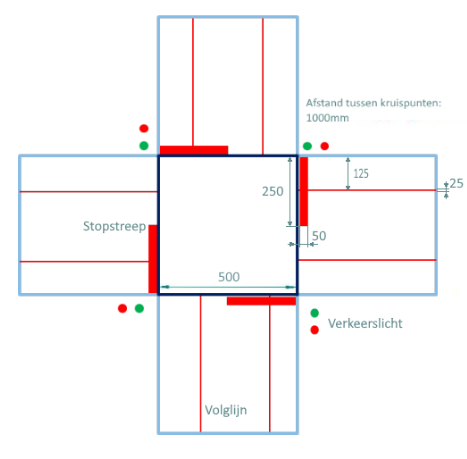
\includegraphics[width = 0.9 \textwidth]{bovenaanzichtkruispunt}
		\cite{kruispunt}
		
	\end{minipage}\hfill
\end{frame}

\section{Oplossing}

\begin{frame}
	\frametitle{Budget}
	\begin{center}
		
		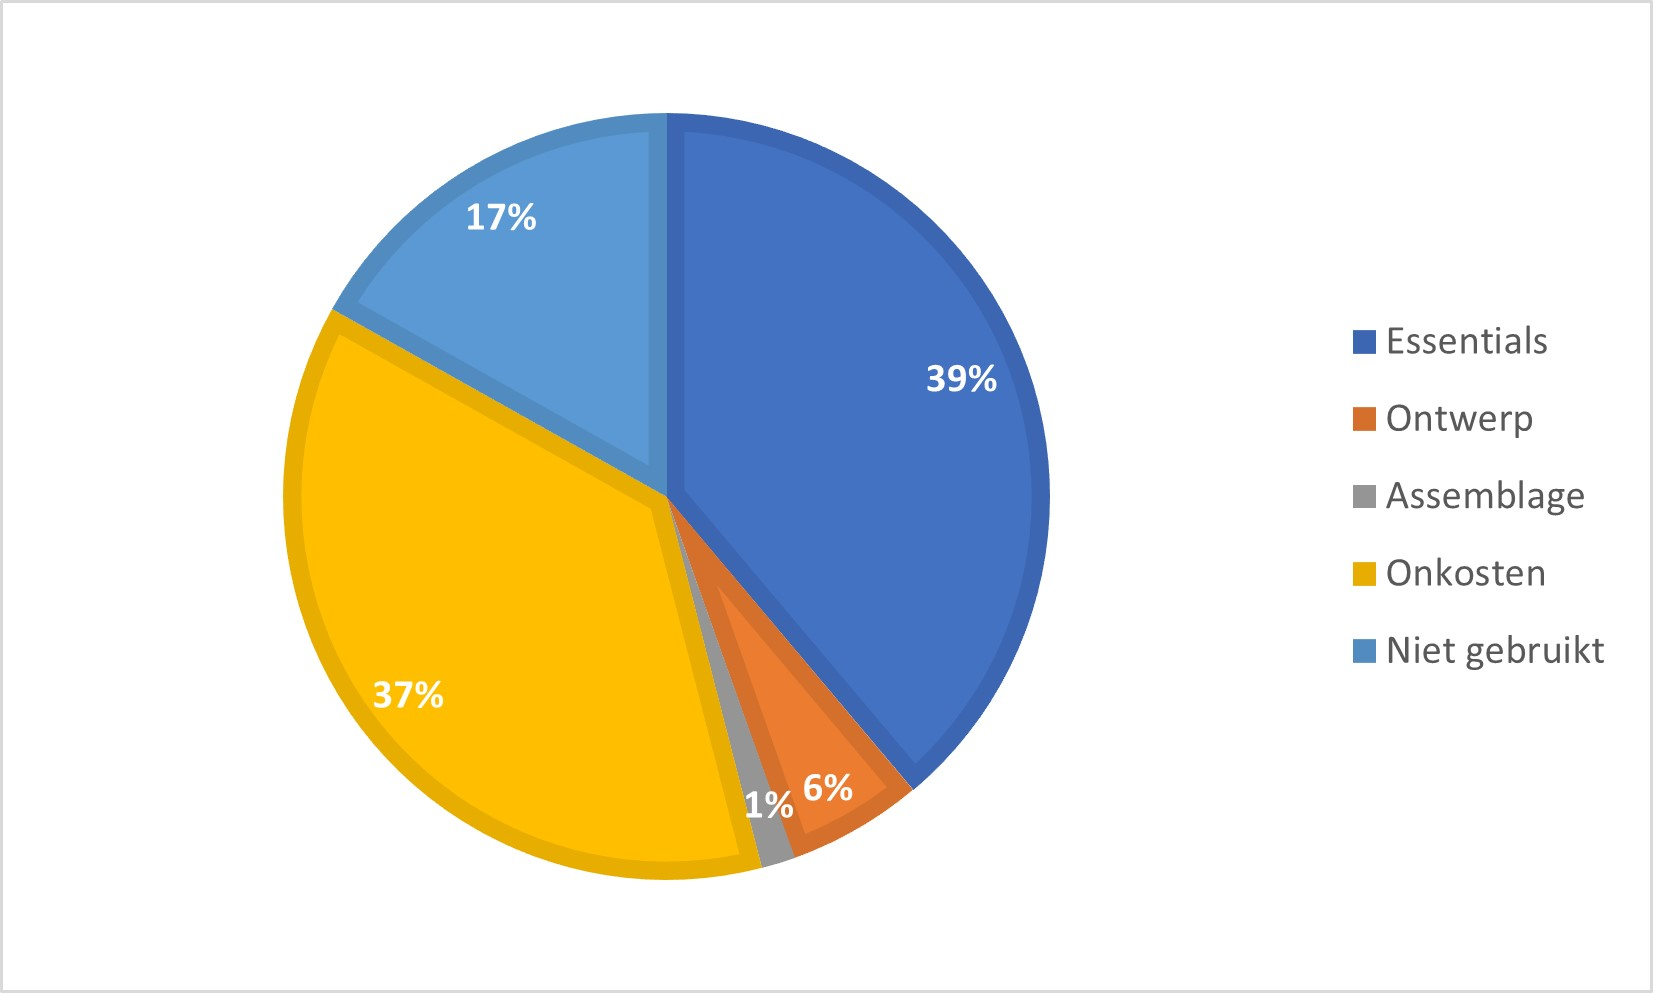
\includegraphics[width = 0.7 \textwidth]{pie}
		
	\end{center}
\end{frame}

\section{Conclusie}
\begin{frame}
\frametitle{Afsluitende frame}
Afsluitende tekst.
\end{frame}

\begin{frame}
	\frametitle{Referenties}
	\bibliographystyle{amsalpha}
	\bibliography{bibliografie_presentatie}
\end{frame}

\end{document}
